\documentclass{article} % Sets what kind of document (book, article, presentation, ...)

%----------
% Packages
%----------
\usepackage{amsmath}	% Allows math environments
\usepackage{amssymb}	% Adds math symbols
\usepackage{setspace}	% For line spacing
\usepackage{hyperref}	% For links
\usepackage{xcolor}     % For colored text
\usepackage{graphicx}   % For images
\usepackage[margin=1in]{geometry} % For margins

\newcommand*\red{\color{red}}  % Add short command for coloring text
\newcommand{\E}{\mathbb{E}}    % Add short command for expectations

%----------
% Title info
%----------
\author{Luke Sonnet}
\title{Probability Review}

%----------
% Body
%----------
\begin{document}

\singlespacing
\maketitle % Make title, will build date, title, author
\onehalfspacing

Much of the language and structure is borrowed from Teppei Yamamoto. This is not meant to be comprehensive but just to get you thinking in these terms. Review your 200A notes and check out the Aronow and Miller 2015 textbook.

\section{Basic Probability Theory}

We have a {\red sample space} $\Omega = \{A, B, \dots\}$. The sample space contains all possible events or outcomes of an experiment or data generating process. If we are considering a coin-toss, then $\Omega = \{H, T\}$ where the outcomes can either be heads or tails. We use probability, and specifically {\red probability functions} to tell us the probability of each event. Following Chad's notation, we can write $p(A)$ to denote the probability function that tells us the probability of event $A$.

I'm not going to cover basic set theory operations. Review your 200A notes. But given this set-up, we can formally define a probability function $p(\cdot)$ as a function that is defined over all subsets of a sample space $\Omega$ and that satisfies three probability axioms:

\begin{enumerate}
	\item {\red Nonnegativity} - $p(A) \geq 0$ for all $A$ in the set of all events $\Omega$
	\item {\red Normalization} - $p(\Omega) = 1$
	\item {\red Additivity} - if $A_1, A_2, \dots$ are disjoint then $p(A_1 \cup A_2 \cup \cdots ) = p(A_1) + p(A_2) + \dots$
\end{enumerate}

Now I'm going to discuss random variables, leaving the discussion of conditional and marginal probabilities for that context.

\section{Random Variables}

Dealing with events is difficult when there become many possible events. For coin tosses, events can be easy, for today's temperature, the events may be infinite since temperature is continuous. 

A {\red random variable} $X$ is a real-valued function that maps the sample space to real numbers, $X : \Omega \rightarrow \mathbb{R}$. In other words, a random variable is a function that returns a real number to each of the outcomes of the experiment, or events in the sample space.

Imagine a coin toss:
\[
X = \begin{cases}
	0 \;\; \text{ if we get tails} \\
	1 \;\; \text{ if we get heads}
\end{cases}
\]

The {\red probability mass function} (or probability discrete function for continuous random variables), assigns probability for each realized value $x \in X$. It is often written as $f_X(x)$; Chad uses $p(x)$. It will follow the probability axioms.

If our coin is fair, then
\[
p(x) = \begin{cases}
1/2 \;\; \text{ if } x = 0 \\
1/2 \;\; \text{ if } x = 1
\end{cases}
\]

This can be simplified as 
\[
p(x) = 0.5 \;\; \forall \; x \in X
\]

A {\red continuous random variable} has a continuous range of possible realizations, or outcomes. If $X$ is a continuous random variable, then it is characterized by a {\red probability density function} that Chad would write as, again $p(x)$.
\[
\text{Pr}(a \leq X \leq b) =  \int_a^b p(x) \, dx
\] 

For a uniform distribution that ranges from $0$ to $4$, we can write it as $X \sim Uniform(0, 4)$. The the probability density function of $X$ is
\[
p(x) = \begin{cases}
1/4 \;\; 0 \leq x \leq 4 \\
0 \;\; \text{otherwise}
\end{cases}
\] 

We commonly work with the normal distribution, which can be described by its mean and variance. We often write $X \sim N(\mu, \sigma^2)$. The PDF of $X$ is

\[
p(x) = \frac{1}{\sigma \sqrt{2\pi}} e^{\frac{(x - \mu)^2}{2\sigma^2}}
\]

So this function is fully described by $\mu$ and $\sigma$. Let $X \sim N(1, 9)$, then our PDF is

\[
p(x) = \frac{1}{3\sqrt{2\pi}} e^{\frac{(x - 1)^2}{18}}
\]

If we sample $10,000$ times from this distribution, we can plot the data using the following distribution:
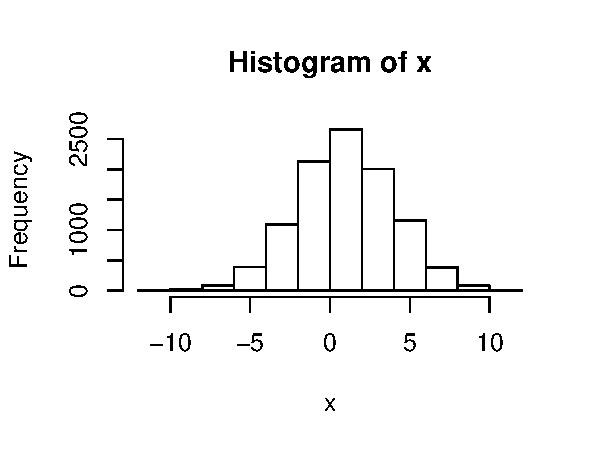
\includegraphics[scale=1]{normal.pdf}

\section{Expectation}

One way to describe a random variable is by its expectation, which can also be considered as it's center of gravity. For a discrete random variable $X$, it is the sum of all of the possible realizations of $X$, $x \in X$ multiplied by the probability of those realizations.

\[
\E[X] = \sum_{x \in X} x p(x)
\]

If we want to consider what happens when we take the expectation of $X$ times some constant $a$, we just have to consider how it changes the right hand side of that equation. Because $a$ is constant, the probabilities will not change, simply the realizations $x\in X$ will change.
\begin{align*}
	\E[aX] &= \sum_{x \in X} ax p(x) \\
	&= a \sum_{x \in X} x p(x) \\
	&= a \E[X]
\end{align*}

Similarly, if $b$ is a constant as well,
\begin{align*}
	\E[aX + b] &= \sum_{x \in X} (ax + b) p(x) \\
	&= \sum_{x \in X} ax p(x) + b p(x) \\
	&= \sum_{x \in X} ax p(x) + \sum_{x \in X} b p(x) \\
	&= a \sum_{x \in X} x p(x) + b \sum_{x \in X} p(x) \\
	&= a \E[X] + b
\end{align*}

Here we use the fact that $\sum_{x \in X} p(x) = 1$, meaning the sum of the probability of all possible realizations of $X$ equals 1. This all is very similar to continuous distribution, although instead of summing over possible realizations of $X$, we integrate over the range of possible $x$ values.

\section{Joint Distributions}

Head over to Teppei Yamamoto's slides.

\end{document}
